\subsection{Komponentbeskrivelse}\label{sec:blockdescription}
Her beskrives komponenterne som blev vist på blokdiagrammet på side~\pageref{fig:blockdiagram}. 

\subsubsection{Bruger}
Brugeren af systemet vil være interesseret i at kunne indhente forskellige målinger fra et system, som kan være placeret på en vilkårlig position, så længe der er mobildækning.

\subsubsection{MC35}
En Siemens MC35 GSM/GPRS Modem (vist på figur~\ref{fig:devicegsm}) er i projektet anvendt til at sende og modtage sms beskeder, som gør kommunikation mellem bruger og system mulig. Under udvikling har to forskellige enheder været brugt. Med den første enhed var der en del inkonsistens i opførsel under udvikling, men da denne enheds blev udskiftet stoppede problemerne og debugging af problemer blev meget lettere.

\begin{figure}[h]
	\centering
	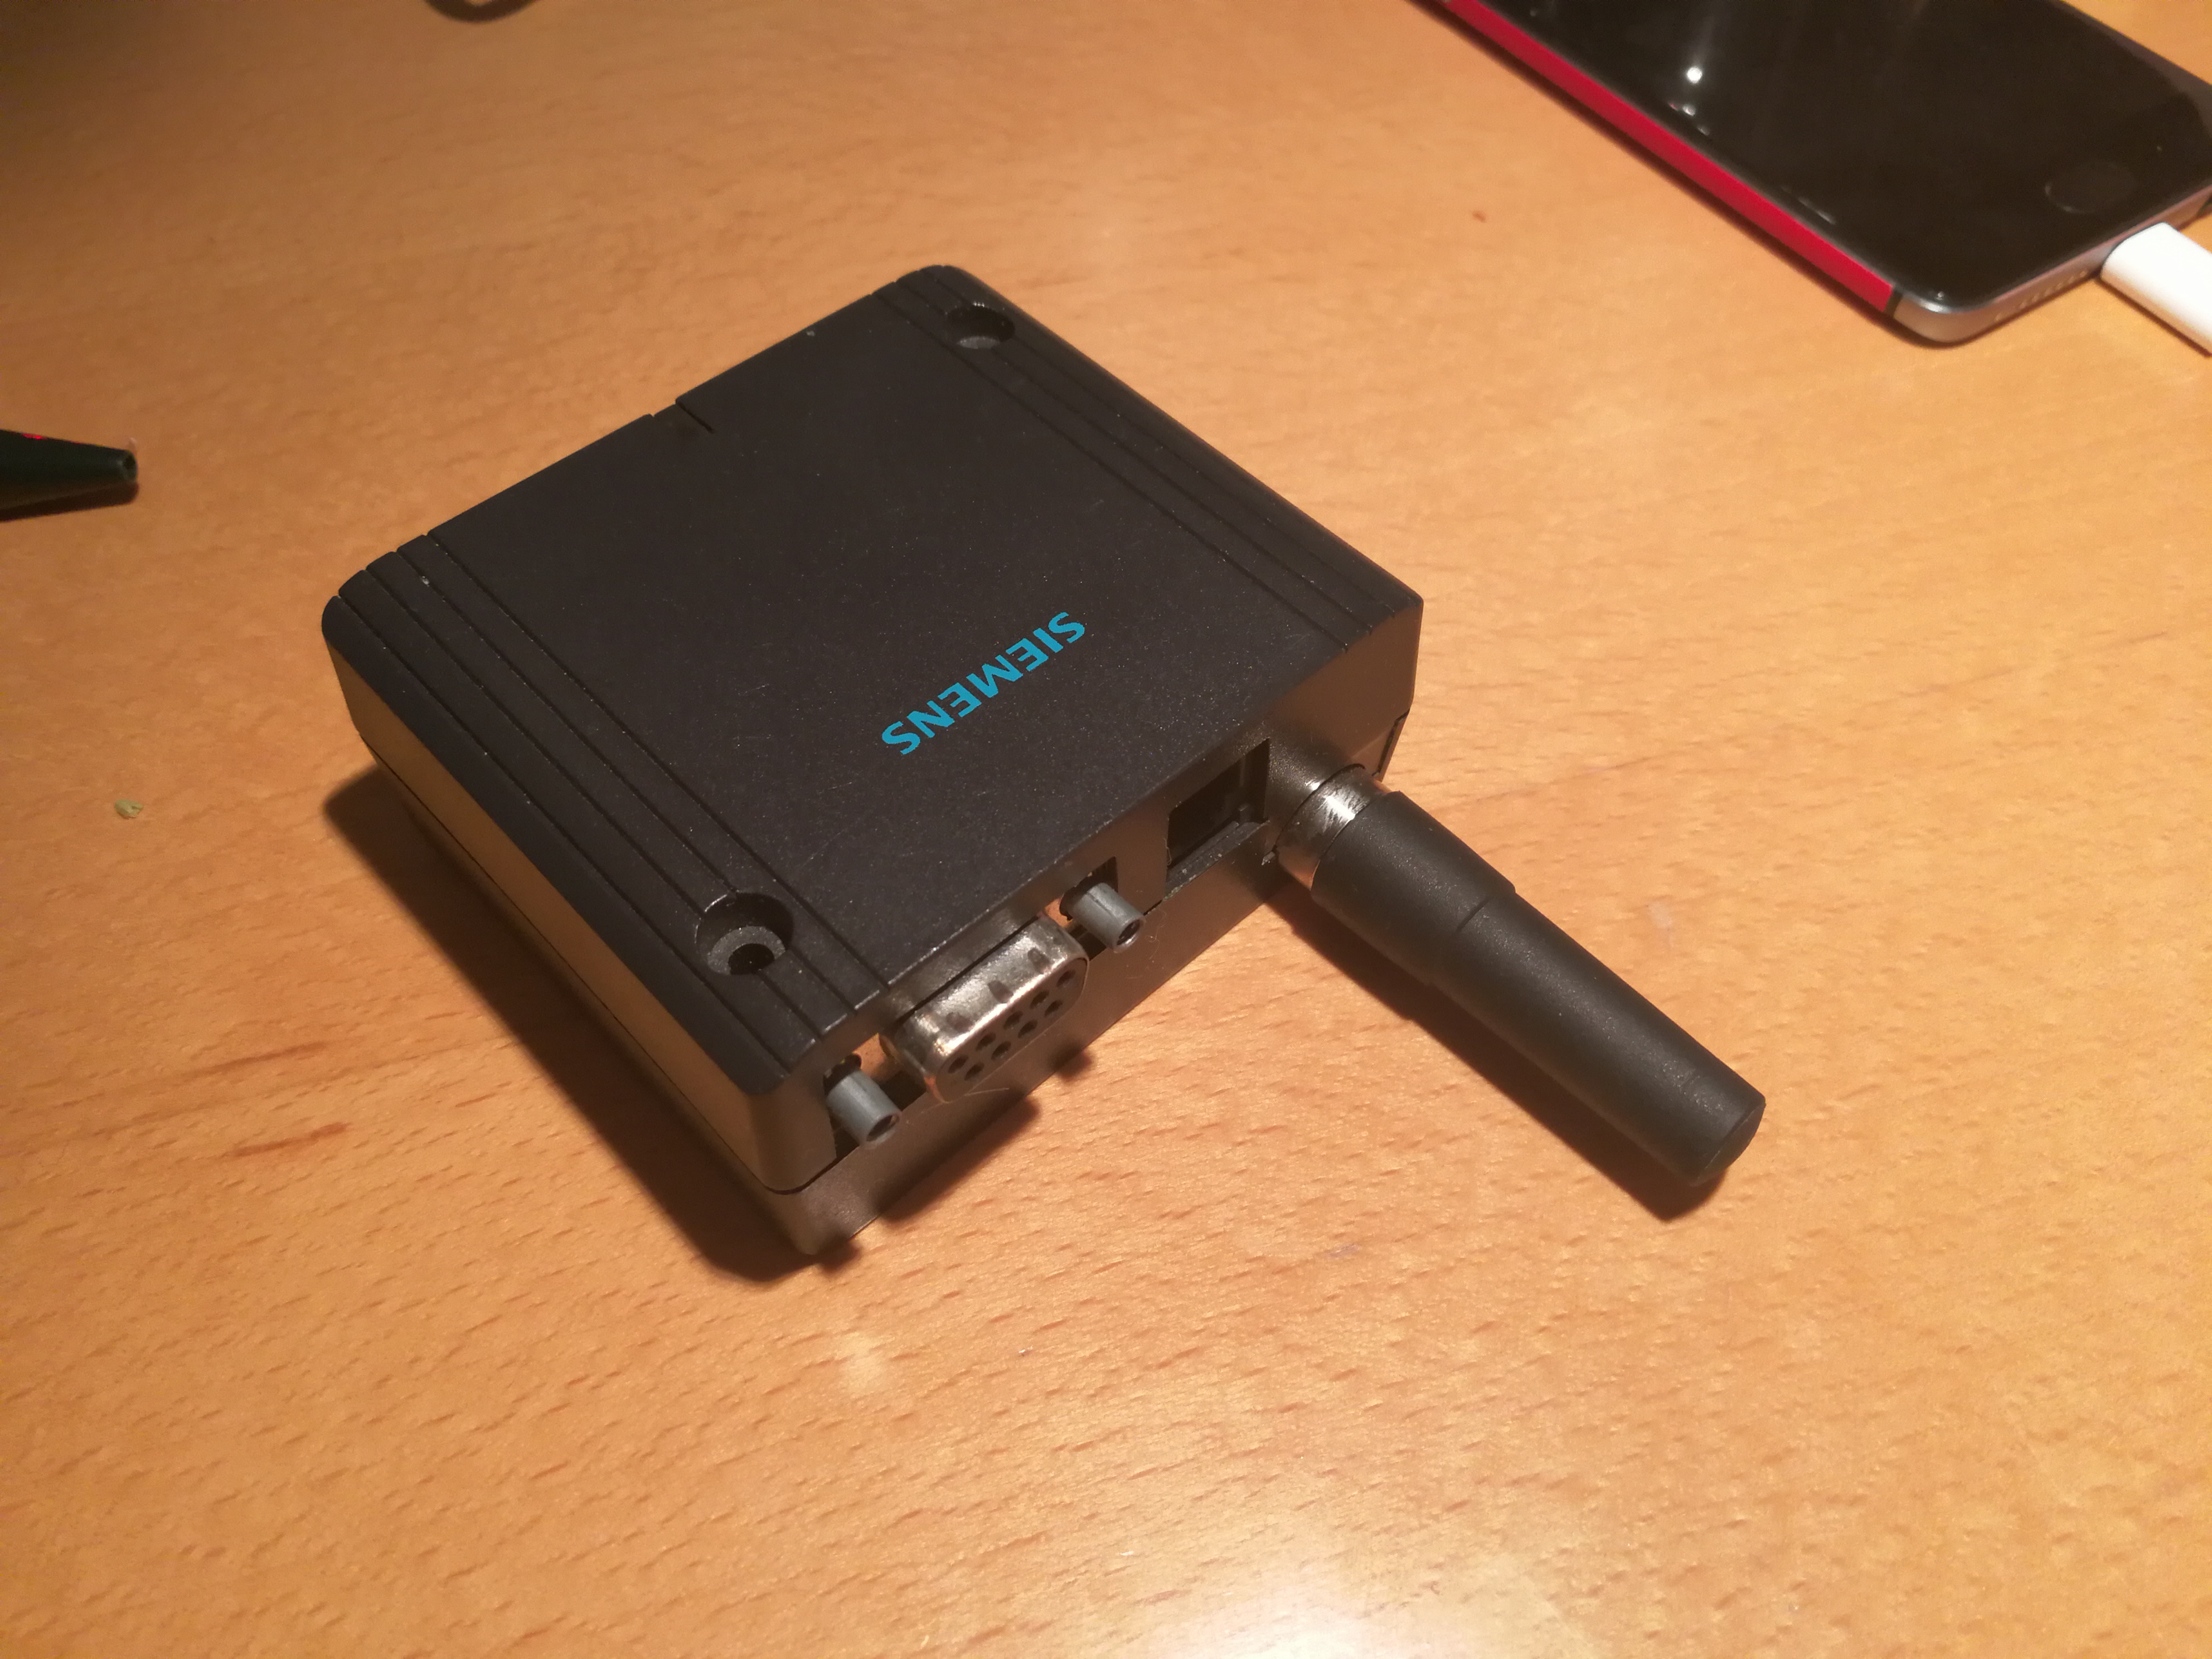
\includegraphics[width=0.7\linewidth]{figs/device_gsm.jpg}
	\caption{Siemens MC35 GSM/GPRS modem.}
	\label{fig:devicegsm}
\end{figure}

Der interfaces mellem ATmega32 og MC35 ved hjælp af en UART forbindelse med en baudrate\footnote{Symboler (signalpulser) per sek.} på 38400.
MC35 har autobauding slået til som fabriks indstilling, hvilket gør det muligt at kommunikere med modemet en række forskellige understøttede hastigheder.
Med autobauding er der dog nogle særlige restriktioner og forudsætninger der skal overholdes:

\begin{itemize}
	\item 3 til 5 sek. delay før den første char i en kommando sendes.
	\item 8 data bits operation, ingen paritet og 1-bit stop.
\end{itemize}

Ved initiering af ATmega32s USART, konfigureres registret UCSRB\footnote{USART Control and Status Register B} 
som kan ses på figur~\ref{fig:regucsrb}. Da der i dette projekt benyttes et interrupt på RXC flaget initieres RXCIE også.
I tabel~\ref{fig:ucszbitsettings} ses data bit konfigurationerne. Da $UCSZ0=1$, $UCSZ1=1$ og $UCSZ2=0$ er default værdier på 
ATmega32 skal de ikke ændres på.

% Added custom table below
%\begin{figure}[h]
%	\centering
%	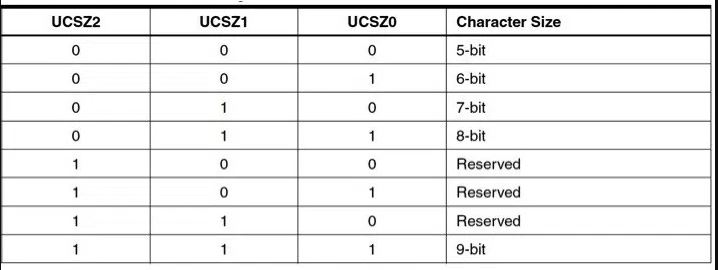
\includegraphics[width=0.7\linewidth]{figs/ucsz_bitsettings.jpg}
%	\caption{UCSZ bit settings på ATmega32.}
%	\label{fig:ucszbitsettings}
%\end{figure}

\begin{table}[h]
	\centering
	\begin{tabular}{|c|c|c|l|}
		\hline
		\rowcolor[HTML]{EFEFEF} 
		\textbf{UCSZ2} & \textbf{UCSZ1} & \textbf{UCSZ0} & \textbf{Character Size} \\ \hline
		0 & 0 & 0 & 5-bit \\ \hline
		0 & 0 & 1 & 6-bit \\ \hline
		0 & 1 & 0 & 7-bit \\ \hline
		0 & 1 & 1 & 8-bit \\ \hline
		1 & 0 & 0 & Reserved \\ \hline
		1 & 0 & 1 & Reserved \\ \hline
		1 & 1 & 0 & Reserved \\ \hline
		1 & 1 & 1 & 9-bit \\ \hline
	\end{tabular}
	\caption{UCSZ bit settings på ATmega32.}
	\label{fig:ucszbitsettings}
\end{table}

Se kodeudsnit~\ref{code:initucsrb} for initiering af USARTen. 

Som nævnt sættes RXC interrupt flaget når der modtages data fra MC35.
Der er skrevet en Interrupt Service Routine der gemmer den modtagne data i et char* array, hvorefter programmet på ATmega32 behandler dataen
og reagerer på eventuelle kommandoer. Hver gang en dataen er behandlet, slettes indholdet af arrayet og er derfor klargjort til næste 
kommando. 

\begin{lstlisting}[caption=Initiering af UCSRB.,label=code:initucsrb] 
	UCSRB = ( (1<<TXEN) | (1<<RXEN) | (1<<RXCIE) );
\end{lstlisting}

\begin{figure}[h]
	\centering
	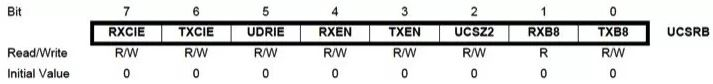
\includegraphics[width=\linewidth]{figs/avr_register_ucsrb.jpg}
	\caption{ATmega32 UCSRB register.}
	\label{fig:regucsrb}
\end{figure}

MC35 sender ''OK'' tilbage efter hver succesfuldt udført kommando, hvilket gør det lettere at reagere på eventuelle fejl fra modemet. En yderligere timing foranstalting er dog at et delay på minimum 200ms køres
 før der igen kan skrives til MC35 efter den har sendt ''OK''. 


\subsubsection{ATmega32}
ATmega32 er brugt sammen med STK500 boardet, som hovedkomponent i udviklingen. Denne er vist på figur~\ref{fig:deviceatmege32}. 
Boardet interfacer som tidligere beskrevet med GSM modemet via UART og fortolker de modtagne kommandoer før der kan anmodes om de ønskede målinger fra BMP modulet, som interfaces med I2C two-wire kommunikation.
STK500 har gjort det markant lettere at udvikle til ATmega32, idet megen funktionalitet er samlet og ikke skal klattes sammen på et fumlebræt. I forbindelse med BMP085 er der lavet en simpel
 spændingsdeler der sørger for at bringe STK500's 5V spænding ned på ca. 3.3V som er angivet i BMP085's datablad.

\begin{figure}[h]
	\centering
	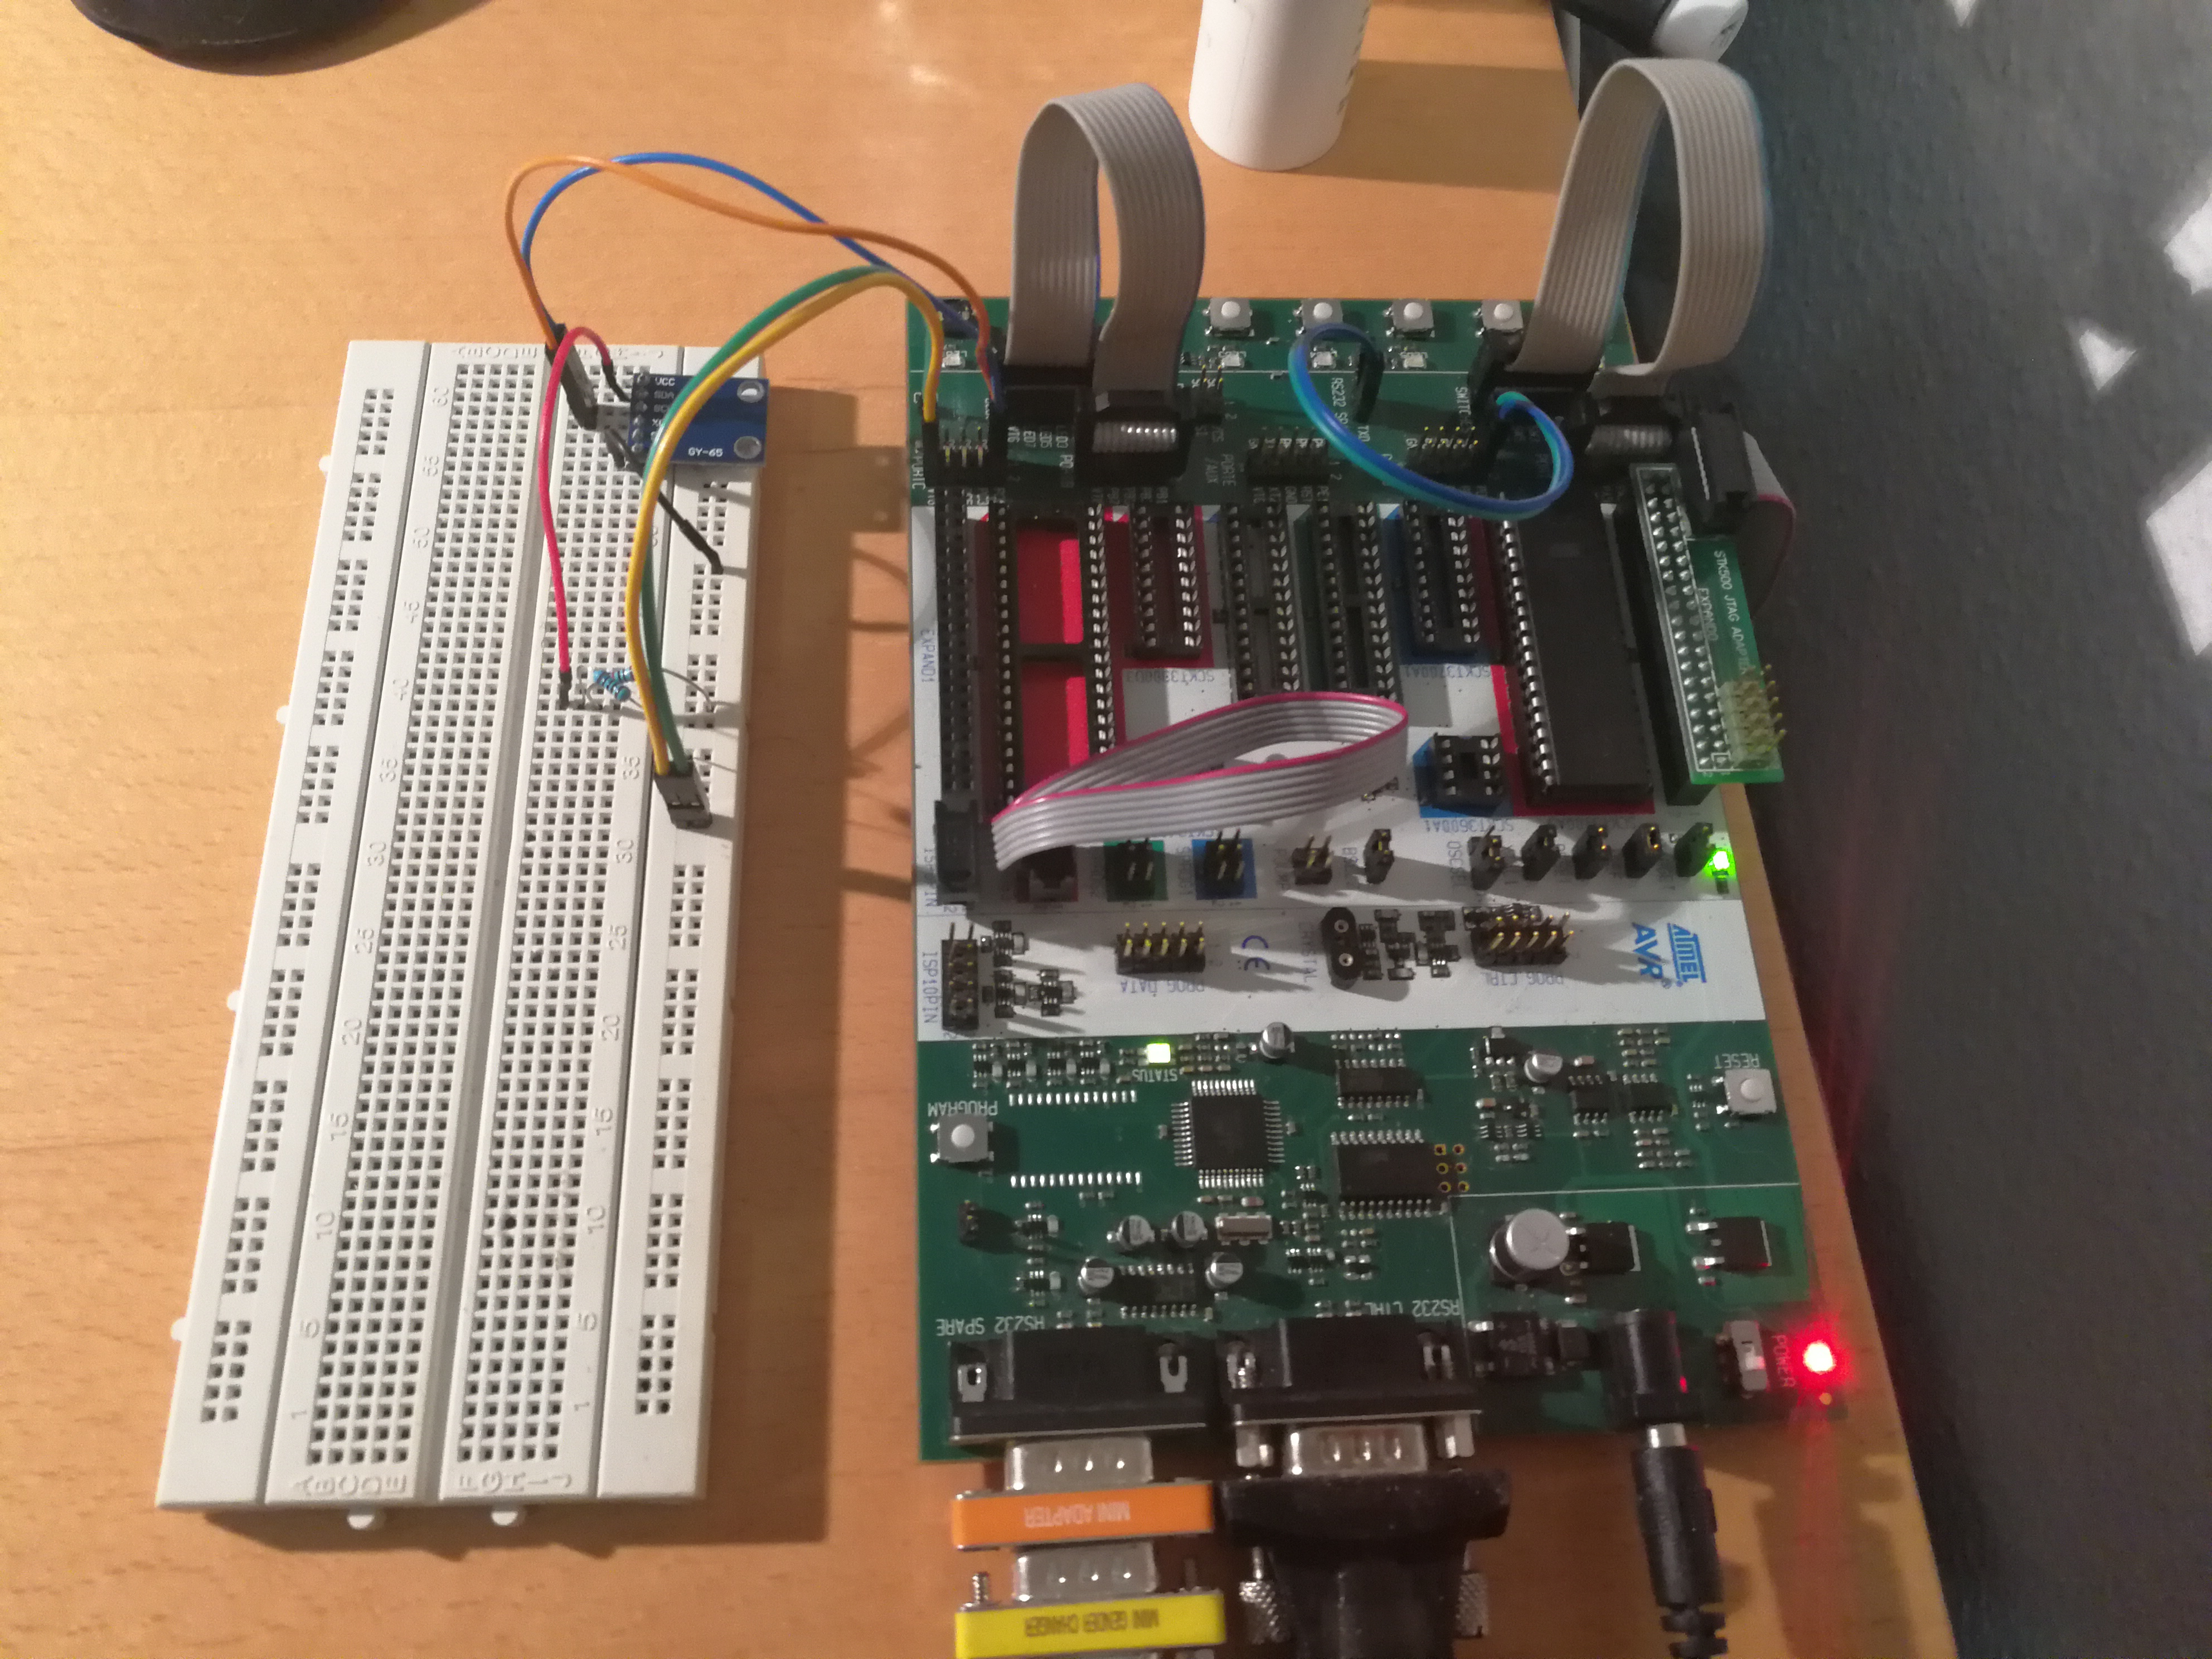
\includegraphics[width=0.7\linewidth]{figs/device_atmega32.jpg}
	\caption{STK500 board opsætning med ATmega32 og BM085.}
	\label{fig:deviceatmege32}
\end{figure}

\subsubsection{BMP}
BMP08 modulet er brugt til at foretage målingerne og kommunikerer med ATmega32 over I2C. Den er i stand til at måle temperatur, lufttryk og altitude. 
Disse tre forskellige målinger kan så anmodes af ATmega32 og senders ud til brugeren. Vist på figur~\ref{fig:devicebmp}.

\begin{figure}[h]
	\centering
	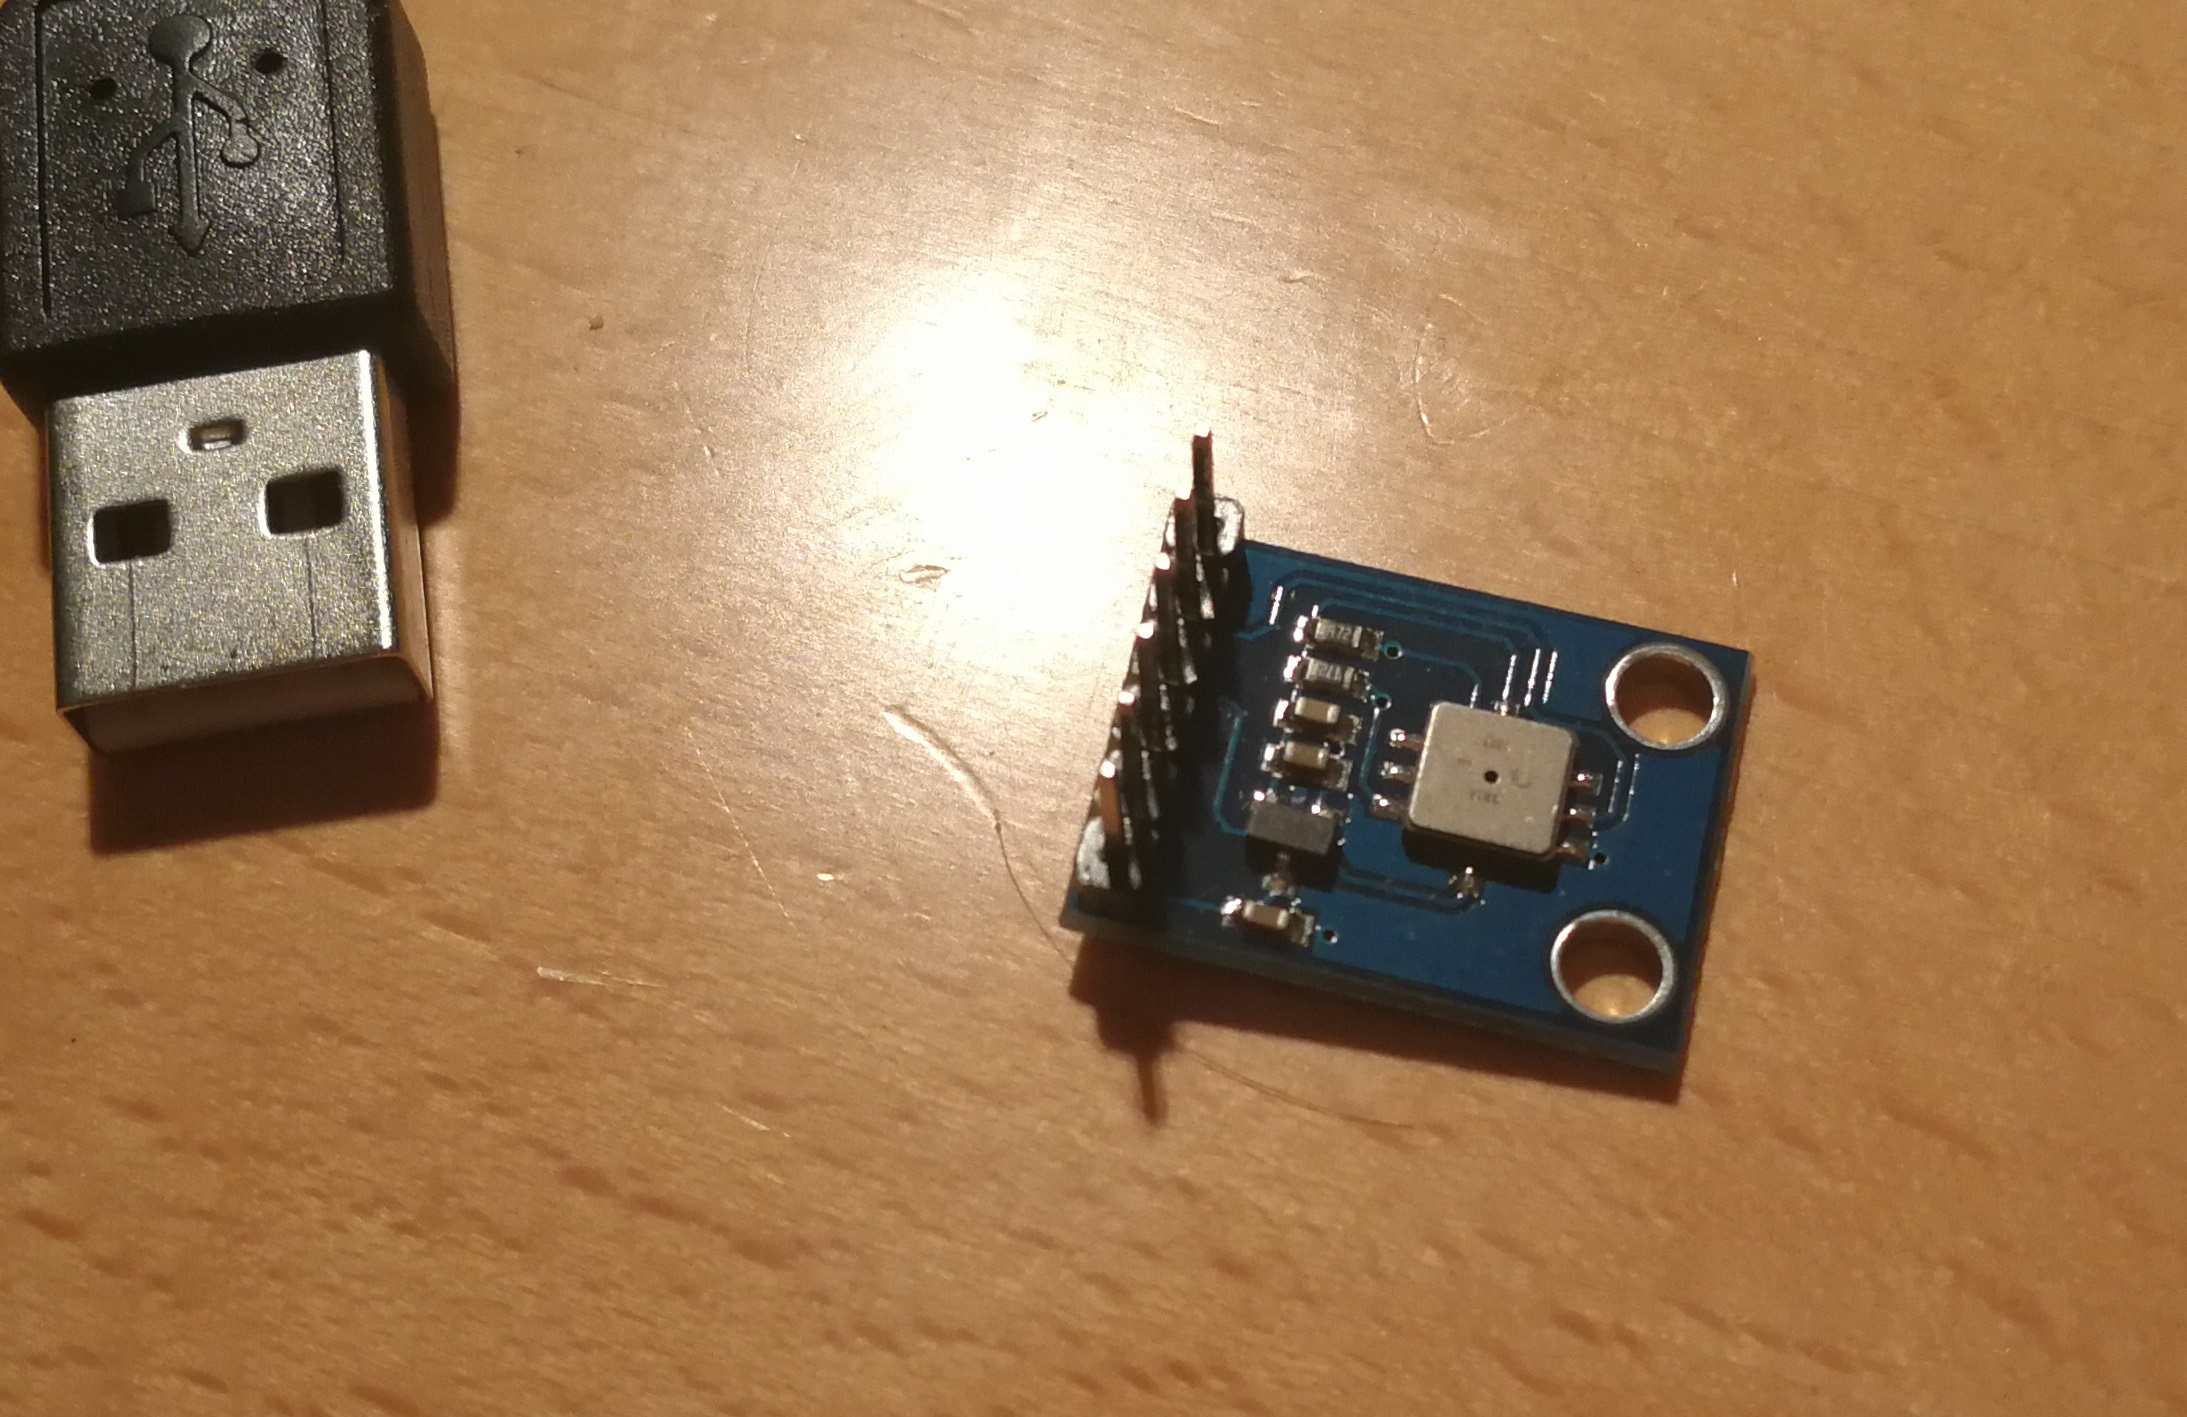
\includegraphics[width=0.7\linewidth]{figs/device_bmp.jpg}
	\caption{BMP085 digital trykføler.}
	\label{fig:devicebmp}
\end{figure}

I forbindelse med BMP085 er der taget udgangspunkt i en driver\footnote{Davide Geroni, 2012} der er afledt af en lignende driver til Arduino.
Driveren bruges i projektet til at hente kalibreringsdata fra BMP085's EEPROM og udføre beregninger på rå måledata. Samtidig giver driveren 
mulighed for udnytte BMP085 chippens forskellige muligheder for målepræcision og oversampling. Da dette projekt ikke nødvendigvis er tidskritisk er 
den højeste målepræcision valgt, dog på beskostning af svartider og strømforbrug.
I forbindelse med brugen af BMP085 er der gjort nogle tekniske overvejelser for at imødekomme sensorens tekniske krav. Disse beskrives nærmere i afsnittet om tekniske overvejelser.
